\documentclass[a4paper,12pt]{article}
\usepackage[T2A]{fontenc}
\usepackage[utf8]{inputenc}
\usepackage[english,russian]{babel}
\usepackage{listings}

\usepackage[table]{xcolor}

\usepackage{amsmath}
\usepackage{MnSymbol}
\usepackage{wasysym}
\usepackage{indentfirst}
\usepackage[unicode, pdftex]{hyperref}

\usepackage{pgfplots}
\pgfplotsset{compat=1.9}

\usepackage{geometry}
\geometry{left=2cm}
\geometry{right=1.5cm}
\geometry{top=1cm}
\geometry{bottom=2cm}

\usepackage{graphicx}
\graphicspath{{img/}}
\DeclareGraphicsExtensions{.pdf,.png,.jpg}

\usepackage{float}

\newcommand{\anonsection}[1]{\section*{#1}\addcontentsline{toc}{section}{#1}}

% переименовываем  список литературы в "список используемой литературы"
\addto\captionsrussian{\def\refname{Список используемой литературы}}

\lstset{
    language=C++,
    numbers=left,
    frame=single,
    texcl=true,
    basicstyle=\ttfamily
}

\begin{document}

\begin{titlepage}

    \begin{center}
        \large
        Государственное образовательное учреждение высшего профессионального образования\\
        “Московский государственный технический университет имени Н.Э.Баумана”
        \vspace{3cm}

        \textsc{Дисциплина: Анализ алгоритмов}
        \vspace{0.5cm}

        \textsc{Лабораторная работа №6}
        \vspace{3cm}

        {\LARGE РЕШЕНИЕ ЗАДАЧИ КОММИВОЯЖЕРА}
        \vspace{3cm}

        Студент группы ИУ7-53,\\
        Степанов Александр Олегович
        \vfill
    \end{center}

    \begin{flushright}
        \begin{tabular}{l}
            Преподаватели:\\
            Строганов Юрий Владимирович\\
            Волкова Лилия Леонидовна
        \end{tabular}
    \end{flushright}

    \begin{center}

        2019 г.

    \end{center}

\end{titlepage}

\tableofcontents

\newpage
\anonsection{Введение}

Задача коммивояжера занимает особое место в комбинаторной оптимизации и исследовании операций.
Исторически она была одной из тех задач, которые послужили толчком для развития этих направлений.
Простота формулировки, конечность множества допустимых решений, но колоссальные затраты на полный
перебор до сих пор подталкивают к разработке все новых и новых численных методов.

С точки зрения практического применения, она не представляет интерес.
Куда важнее дополнения задачи для транспорта и логистики, когда несколько
транспортных средств ограниченной грузоподъемности должны обслуживать клиентов,
посещая их в заданные временные окна \cite{kommivoyadjer}.

Целью данной работы является создание приложения для наглядного представления работы муравьиного
алгоритма и для проведения вычислительных экспериментов.

В данной работе ставятся следующие задачи:

\begin{itemize}
    \item изучение существующих алгоритмов задачи коммивояжера;
    \item реализация муравьиного алгоритма;
    \item проведение вычислительного эксперимента.
\end{itemize}

\newpage
\section{Аналитическая часть}

Рассмотрим задачу коммивояжера и пути ее решений.

\subsection{Описание задачи}

Задача коммивояжёра –- одна из самых известных задач дискретной оптимизации. Задача заключается в нахождении
самого выгодного маршрута, проходящего через указанные города хотя бы по одному разу с последующим возвратом
в исходный город \cite{Levitin}.

Постановка задачи коммивояжёра: пусть дана сеть из $N$ городов. Коммивояжёр, выходящий из какого-нибудь города,
желает посетить $N-1$ других городов и вернуться в изначальный пункт. Расстояния между всеми этими городами
известны. Требуется установить, в каком порядке коммивояжёру следует посетить города, чтобы суммарное пройденное
расстояние было минимальным.

\subsection{Пути решения}

Для решения задачи коммивояжера разработаны различные алгоритмы:

\begin{enumerate}
    \item метод полного перебора;
    \item жадный алгоритм;
    \item муравьиный алгоритм.
\end{enumerate}

В данной работе проводится исследование двух из них: метода полного перебора и муравьиного алгоритма.

Алгоритм полного перебора осуществляет поиск всех решений путём перебора всех вариантов в количестве $N!$
путей, позволяя получить глобальный минимум по всему графу. Главный недостаток метода полного перебора –- временные затраты.

Муравьиный алгоритм (алгоритм оптимизации подражанием муравьиной колонии) представляет собой имитацию поведения колонии
муравьёв в природе. В основе муравьиного алгоритма лежит вероятностный подход к поиску оптимального пути, однако имеют
большое значение дополнительные критерии.

Преимуществами алгоритма являются невысокая погрешность найденного решения, низкие временные затраты при работе
с графами большой размерности, модифицируемость алгоритма и возможность распараллеливания \cite{ant}.

У муравья есть 3 чувства:

\begin{enumerate}
    \item обоняние -– муравей может чуять феромон и его концентрацию на ребре;
    \item зрение –- муравей может оценить длину ребра;
    \item память –- муравей запоминает посещенные города.
\end{enumerate}

При старте матрица феромонов $\tau$ инициализируется равномерно некоторой константой.
Если муравей $k$ находится в городе $i$ и выбирает куда пойти, то делает это по вероятностному правилу, указанному
на формуле \ref{eq:ant}.

\begin{equation}\label{eq:ant}
    P_{x,y}(t) =
    \begin{cases}
        \frac{\tau_{ij}(t)^\alpha \cdot \nu_{ij}^\beta}{\sum_q^\text{cities} \tau{iq}(t)^\alpha \nu_{iq}^\beta},
        \text{ если город } j \text{ в списке целей} \\
        0, \text{ иначе} \\
    \end{cases},
\end{equation}

где cities -- список посещенных городов, $\alpha, \beta$ -- весовые коэффициенты,
важность феромона и привлекательность ребра соотвественно.

Ночью пересчитываются феромоны по формуле \ref{eq:fer}.

\begin{equation}\label{eq:fer}
    \tau(t+1) = \tau_{ij}(t) \cdot (1 - \rho) + \Delta \tau_{ij}(t)
\end{equation}

\begin{equation}
    \Delta \tau_{ij}(t) = \sum_{k=1}^n \Delta \tau_{k,ij}(t)
\end{equation}

\begin{equation}
    \Delta \tau_{k,ij}(t) =
    \begin{cases}
        \frac{Q}{L_k}, \text{ если ребро } ij \text{ в маршруте } k \text{-го муравья} \\
        0, \text{ иначе} \\
    \end{cases}
\end{equation}

где $L_k$ -- длина маршрута $k$-го муравья, $\rho$ -- коэффициент испарения феромона, $Q$ - нормированная константа
порядка длины наилучшего маршрута

\subsection{Выводы}

Изучив алгоритм муравья, необходимо разработать его и провести исследование.

\newpage
\section{Конструкторская часть}

Рассмотрим алгоритм полного перебора и муравьиный алгоритм.

\subsection{Функциональная модель}

На рисунке \ref{img:idef0} представлена функциональная модель IDEF0
первого уровня, а на рисунке \ref{img:idef0_2} IDEF0 второго уровня.

\begin{figure}[H]
    \centering
    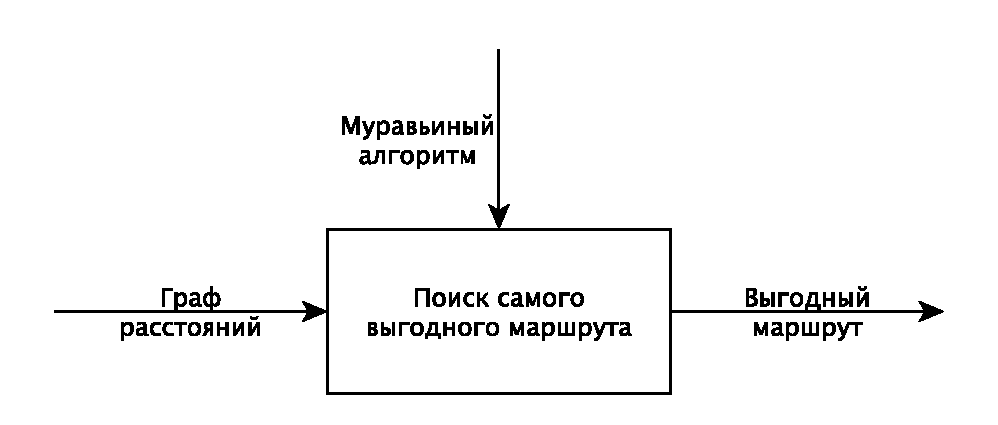
\includegraphics[scale=0.9]{idef0}
    \caption{IDEF0 первого уговня}
    \label{img:idef0}
\end{figure}

\begin{figure}[H]
    \centering
    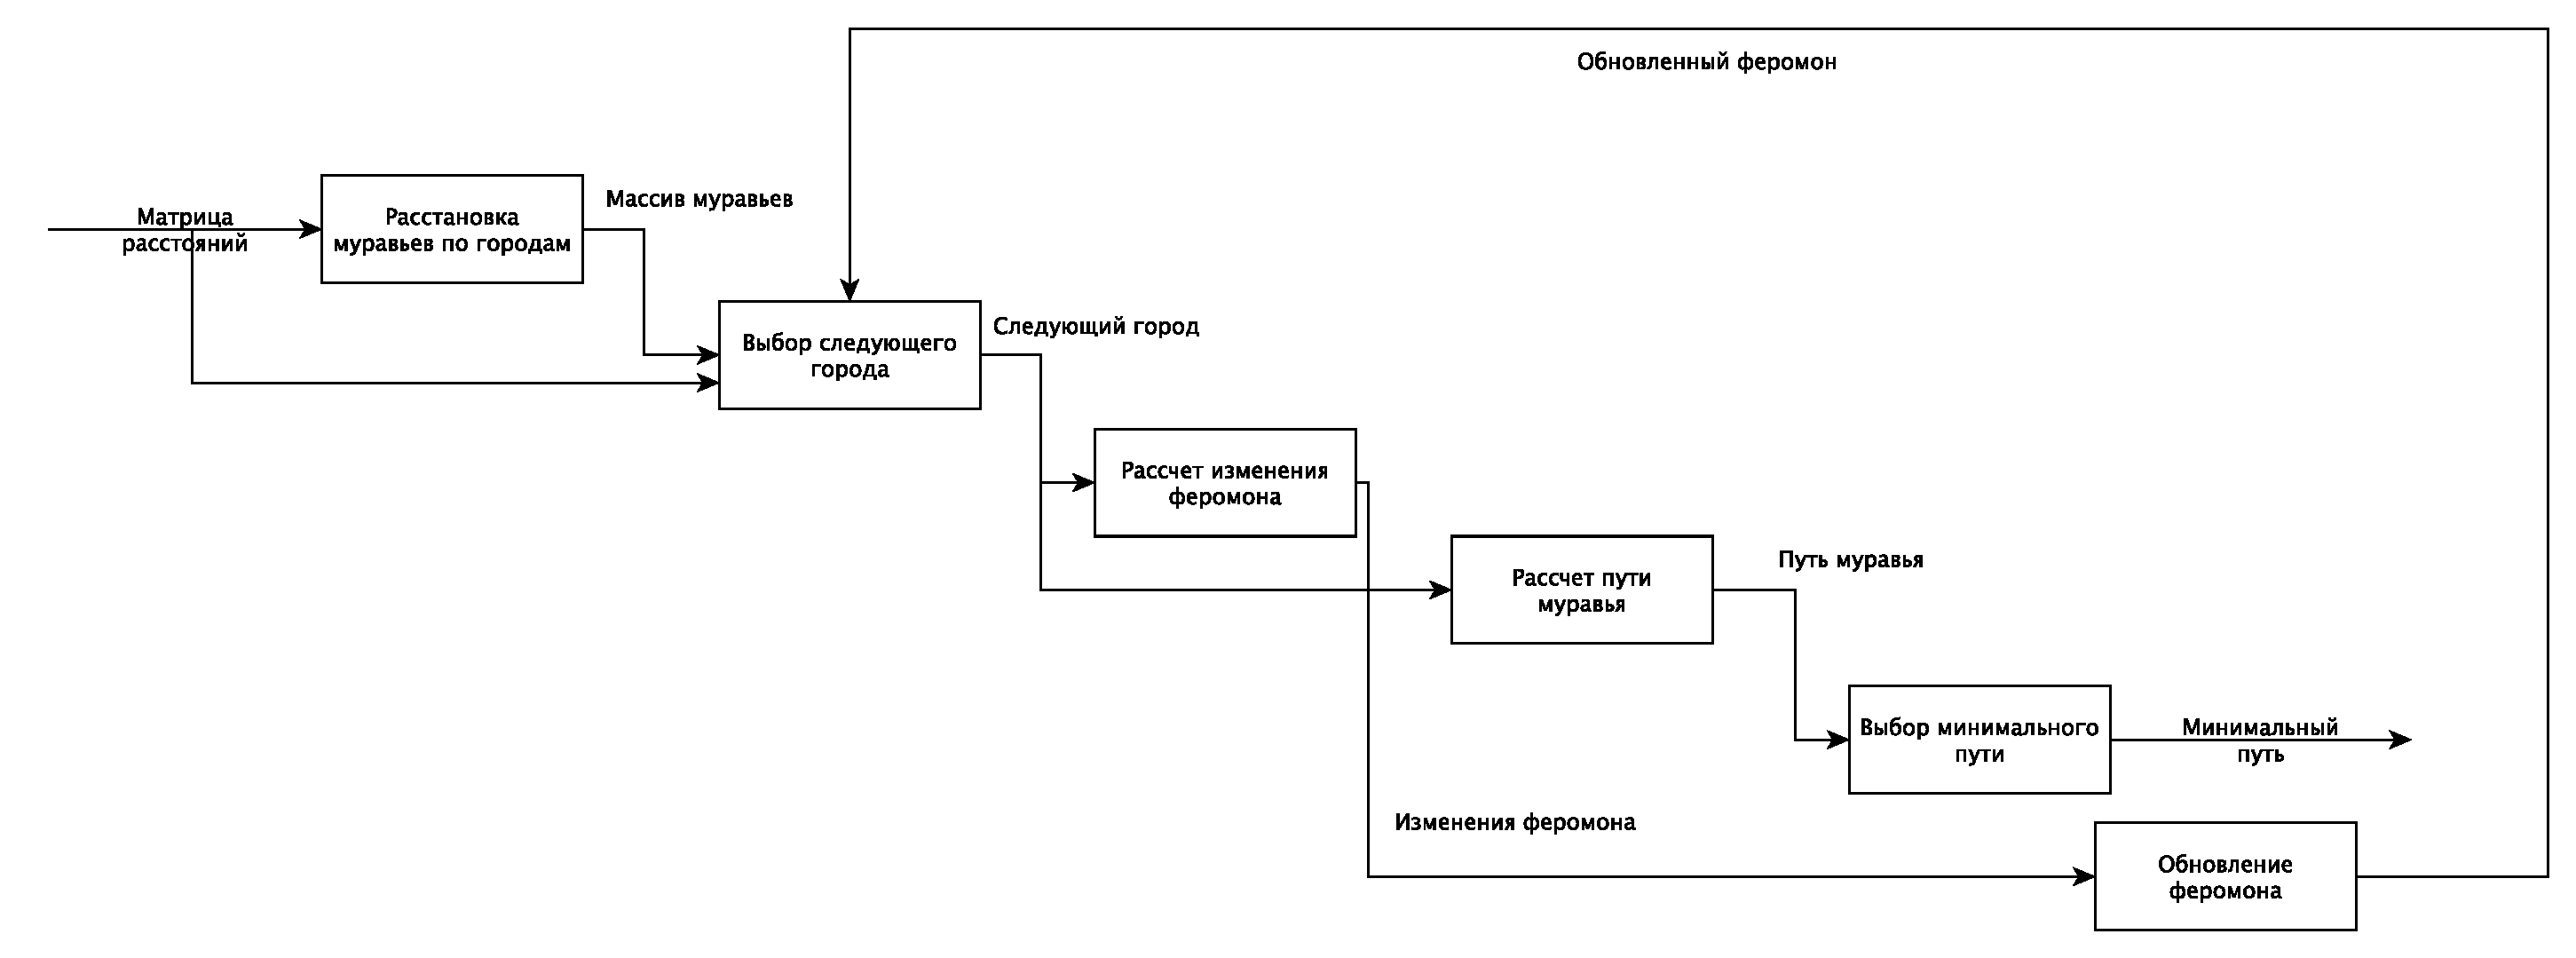
\includegraphics[scale=0.3]{idef0_lvl2}
    \caption{IDEF0 второго уговня}
    \label{img:idef0_2}
\end{figure}

\subsection{Схемы алгоритмов}

На рисунке \ref{img:ant} представлена схема муравьиного алгоритма.

\begin{figure}[H]
    \centering
    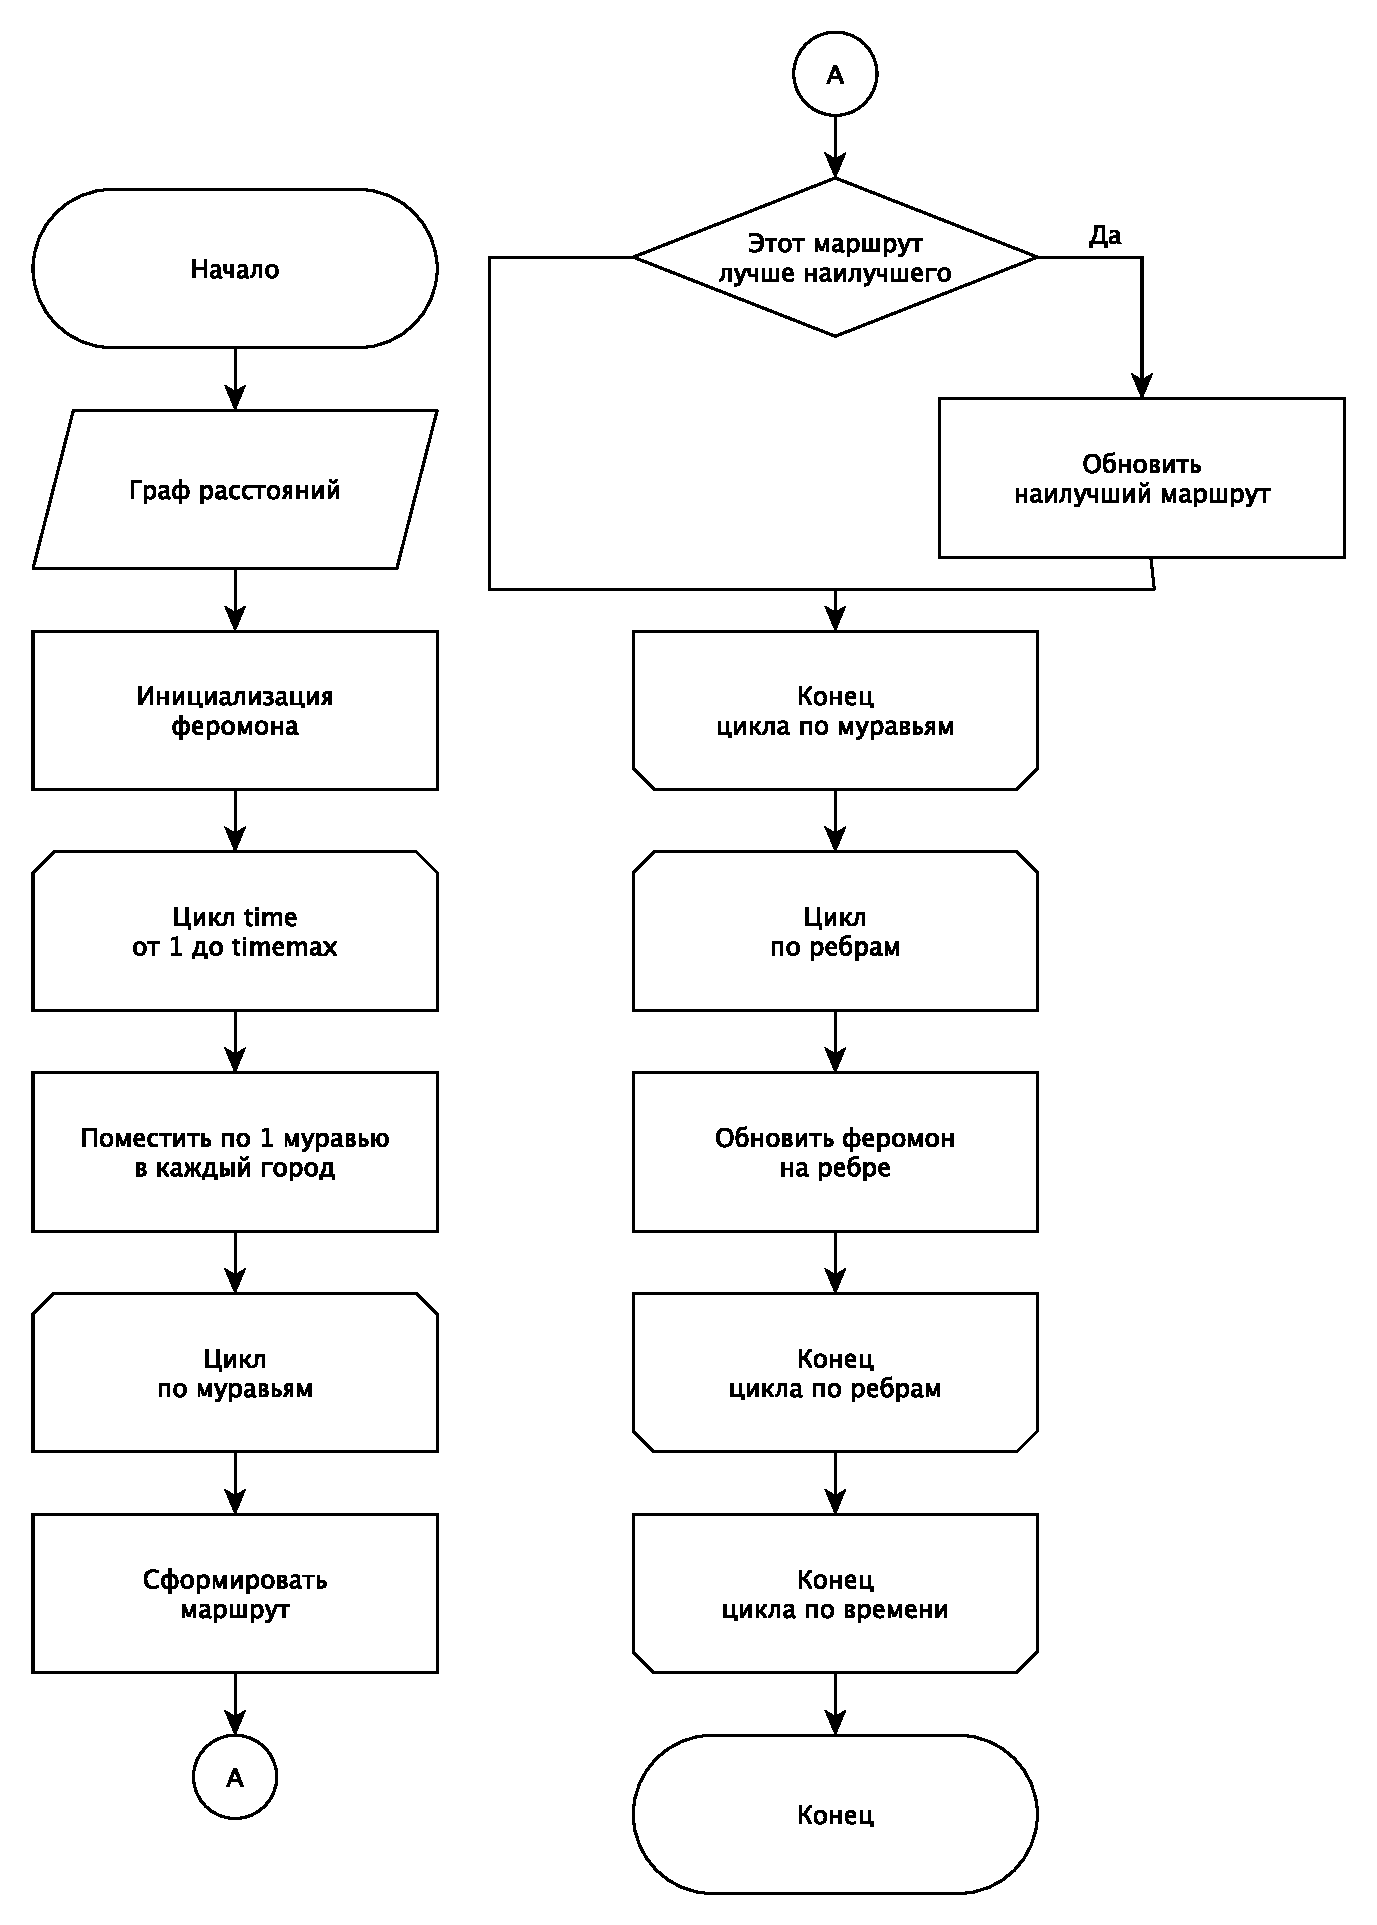
\includegraphics[scale=0.7]{ant}
    \caption{Схема муравьиного алгоритма}
    \label{img:ant}
\end{figure}

\subsection{Выводы}

Необходимо разработать данный алгоритм, провести тестирование и исследование, сравнив с
алгоритмом полного перебора.

\newpage
\section{Технологическая часть}

Реализуем необхоимые алгоритмы.

\subsection{Требования к программному обеспечению}

Программное обеспечение должно предоставлять возможность замера процессорного времени выполнения алгоритмов.
Требуется строить графы для различных данных.

\subsection{Средства реализации}

В качестве языка программирования был выбран {\ttfamily C++}.
Данный язык имеет высокую скорость и богатую стандартную библиотеку,
содержащую необходимые контейнеры для данной работы. Программа, написанная на
{\ttfamily C++}, будет доступна на всех платформах.

\subsection{Листинг кода}

На листингах \ref{lst:fullcall}, \ref{lst:full} и \ref{lst:dist} представлен алгоритм полного рекурсивного
перебора всех путей.

\begin{lstlisting}[caption=Вызов алгоритма рекурсивного перебора,label=lst:fullcall]
std::pair< std::vector< size_t >, size_t > FullSearch::way(
    const Matrix< size_t >& distances)
{
    minDist = -1;

    std::vector< size_t > indexes;
    for (int i = 0; i < distances.size(); ++i)
        indexes.push_back(i);

    recursive(distances, indexes, 1);

    return std::pair< std::vector< size_t >, size_t >(minWay,
                                                      minDist);
}
\end{lstlisting}

\begin{lstlisting}[caption=Алгоритм рекурсивного перебора,label=lst:full]
void FullSearch::recursive(const Matrix< size_t >& distances,
                           std::vector< size_t >& indexes,
                           size_t curIndex)
{
    if (curIndex >= indexes.size()) {
        size_t dist = distance(distances, indexes);

        if (dist < minDist) {
            minDist = dist;
            minWay = indexes;
        }

        return;
    }

    recursive(distances, indexes, curIndex + 1);

    for (int i = curIndex + 1; i < indexes.size(); ++i) {
        std::swap(indexes[curIndex], indexes[i]);
        recursive(distances, indexes, curIndex + 1);
        std::swap(indexes[curIndex], indexes[i]);
    }
}
\end{lstlisting}

\begin{lstlisting}[caption=Подсчет пути,label=lst:dist]
size_t FullSearch::distance(const Matrix< size_t >& distances,
                            const std::vector< size_t >& indexes)
{
    size_t dist = 0;
    for (int i = 0; i < indexes.size() - 1; ++i) {
        dist += distances[indexes[i]][indexes[i + 1]];
    }
    dist += distances[indexes[0]][indexes[indexes.size() - 1]];
    return dist;
}
\end{lstlisting}

На листинге \ref{lst:ant} представлен муравьиный алгоритм.

\begin{lstlisting}[caption=Муравьиный алгоритм,label=lst:ant]
std::pair< std::vector< size_t >, size_t > AntSearch::way(
    const Matrix< size_t >& distances,
    double alpha,
    double beta,
    double rho,
    double tmax)
{
    srand(time(NULL));

    Matrix< double > pheromone(distances.size(), 0.1);

    size_t minDist = -1;
    std::vector< size_t > minWay(distances.size());

    for (int time = 0; time < tmax; ++time) {
        std::vector< int > ants(distances.size());
        std::vector< std::vector< double > > delta;

        for (int i = 0; i < distances.size(); ++i) {
            ants[i] = i + 1;
            delta.push_back(
                std::vector< double >(distances.size())
            );
        }

        for (int ant = 0; ant < ants.size(); ++ant) {
            int count = 0;
            std::vector< int > cities(distances.size());
            std::vector< size_t > way(distances.size());

            cities[ant] = 1;
            way[0] = ant;

            int len = 0;

            while (count + 1 < distances.size()) {
                std::vector< double > p(distances.size());

                for (int j = 0; j < distances.size(); ++j) {
                    if (cities[j] == 0) {
                        p[j] =
                            std::pow(
                                pheromone[way[count]][j],
                                alpha
                            ) *
                            std::pow(
                                distances[way[count]][j],
                                beta
                            );

                        double all = 0;

                        for (int q = 0; q < count; ++q) {
                            all +=
                                std::pow(
                                    pheromone[way[q]][j],
                                    alpha
                                ) *
                                std::pow(
                                    distances[way[q]][j],
                                    beta
                                );
                        }

                        p[j] /= all;
                    } else {
                        p[j] = 0;
                    }
                }

                std::vector< int > arr(
                    distances.size() - count - 1
                );
                int cyc = 0;

                for (int i = 0; i < distances.size(); ++i) {
                    if (cities[i] == 0) {
                        arr[cyc] = i;
                        ++cyc;
                    }
                }

                int rdm = rand() % (distances.size() - count - 1);
                len += distances[way[count]][arr[rdm]];
                ++count;
                way[count] = arr[rdm];
                cities[arr[rdm]] = 1;
            }

            len += distances[way[0]][way[distances.size() - 1]];

            for (int i = 0; i < distances.size() - 1; ++i) {
                delta[way[i]][way[i + 1]] += minDist / len;
                delta[way[i + 1]][way[i]] += minDist / len;
            }

            if (len < minDist) {
                minDist = len;
                minWay = way;
            }
        }

        for (int i = 0; i < distances.size() - 1; ++i) {
            for (int j = i + 1; j < distances.size(); ++j) {
                pheromone[i][j] *= (1 - rho);
                pheromone[i][j] += delta[i][j];
            }
        }
    }

    return std::pair< std::vector< size_t >, size_t >(minWay,
                                                      minDist);
}
\end{lstlisting}

\subsection{Тестирование}

Для тестирования были заготовлены следующие тесты, которые представлены
на таблице \ref{table:test}.

\begin{table}[H]
    \caption{Тесты}
    \label{table:test}
    \centering
    \begin{tabular}{|l||c|}
        \hline
        Входной граф & Ожидаемый результат \\
        \hline
        \hline
        \hline
        4 & \\
        0 1 2 3 & \\
        1 0 3 4 & 0 1 2 3 \\
        2 3 0 5 & dist = 12 \\
        3 4 5 0 & \\
        \hline
        5 & \\
        0 1 -1 3 4 & \\
        1 0 3 4 5 & 0 1 3 4 2 \\
        -1 3 0 5 -1 & dist = 10 \\
        3 4 5 0 7 & \\
        4 5 -1 7 0 & \\
        \hline
        5 & \\
        0 5 8 9 2 & \\
        5 0 3 3 4 & 0 2 1 3 4 \\
        8 3 0 7 6 & dist = 17 \\
        9 3 7 0 1 & \\
        2 4 6 1 0 & \\
        \hline
    \end{tabular}
\end{table}

\subsection{Выводы}

Разаботаны алгоритмы полного перебора и муравьиный алгоритм, необходимо исследовать муравьиный алгоритм
с помощью алгоритма перебора, предварительно его протестировав.

\newpage
\section{Экспериментальная часть}

Необходимо протестировать алгоритм перебора и провести исследование.

\subsection{Примеры работы}

На рисунках \ref{img:zero_arg}, \ref{img:not_exist} и \ref{img:good} представлены примеры работы программы.

\begin{figure}[H]
    \centering
    
\includegraphics[scale=0.4]{zero_arg}
    \caption{Запуск без аргументов}
    \label{img:zero_arg}
\end{figure}

\begin{figure}[H]
    \centering
    
\includegraphics[scale=0.4]{not_exist}
    \caption{Запуск с несуществующим файлом}
    \label{img:not_exist}
\end{figure}

\begin{figure}[H]
    \centering
    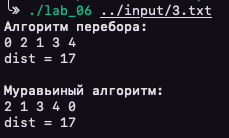
\includegraphics[scale=1]{good}
    \caption{Корректный файл}
    \label{img:good}
\end{figure}

\subsection{Результаты тестирования}

Результаты тестирования представлены на таблице \ref{table:test_result}.

\begin{table}[H]
    \caption{Результаты}
    \label{table:test_result}
    \centering
    \begin{tabular}{|l||c|}
        \hline
        Входной граф & Резуьтат \\
        \hline
        \hline
        \hline
        4 & \\
        0 1 2 3 & \\
        1 0 3 4 & 0 1 2 3 \\
        2 3 0 5 & dist = 12 \\
        3 4 5 0 & \\
        \hline
        5 & \\
        0 1 -1 3 4 & \\
        1 0 3 4 5 & 0 1 3 4 2 \\
        -1 3 0 5 -1 & dist = 10 \\
        3 4 5 0 7 & \\
        4 5 -1 7 0 & \\
        \hline
        5 & \\
        0 5 8 9 2 & \\
        5 0 3 3 4 & 0 2 1 3 4 \\
        8 3 0 7 6 & dist = 17 \\
        9 3 7 0 1 & \\
        2 4 6 1 0 & \\
        \hline
    \end{tabular}
\end{table}

Все тесты пройдены успешно.

\subsection{Выбор коэффициентов}

Проведено исследование сравнения результатов поного перебора с муравьиным алгоритмом с различными
значениями коээфициентов
($0 \le \rho \le 1;\ 0.2 \le \alpha \le 0.8;\ \alpha + \beta = 1;\ 0.2 \le \beta \le 1;\ 10 \le t_{\max} \le 1000$).

$\alpha$ -- коэффициент стадности, $\beta$ -- коэффициент жадности, $t_{\max}$ -- количество итераций времени, $\rho$ -- cкорость
испарения фероменов.

\begin{table}[H]
    \centering
    \caption{5 городов}
    \label{table:city5}
    \begin{tabular}{|c|c|c|c|c|c|}
        \hline
        $\alpha$ & $\beta$ & $\rho$ & $t_{max}$ & Длина маршрута муравья & Длина маршрута перебора \\
        \hline
        0.2 & 0.8 & 0 & 10 & 17 & 17 \\
        0.2 & 0.8 & 0 & 60 & 17 & 17 \\
        0.2 & 0.8 & 0 & 110 & 17 & 17 \\
        0.2 & 0.8 & 0 & 160 & 17 & 17 \\
        ... & ... & ... & ... & ... & ... \\
        0.8 & 0.2 & 1 & 510 & 17 & 17 \\
        0.8 & 0.2 & 1 & 560 & 17 & 17 \\
        0.8 & 0.2 & 1 & 610 & 17 & 17 \\
        0.8 & 0.2 & 1 & 660 & 17 & 17 \\
        \hline
    \end{tabular}
\end{table}

\begin{table}[H]
    \centering
    \caption{8 городов}
    \label{table:city15}
    \begin{tabular}{|c|c|c|c|c|c|}
        \hline
        $\alpha$ & $\beta$ & $\rho$ & $t_{max}$ & Длина маршрута муравья & Длина маршрута перебора \\
        \hline
        0.2 & 0.8 & 0 & 50 & 22 & 22 \\
        0.2 & 0.8 & 0 & 100 & 22 & 22 \\
        0.2 & 0.8 & 0 & 150 & 22 & 22 \\
        0.2 & 0.8 & 0 & 200 & 22 & 22 \\
        0.2 & 0.8 & 0 & 250 & 22 & 22 \\
        0.2 & 0.8 & 0 & 300 & 22 & 22 \\
        0.2 & 0.8 & 0 & 350 & 25 & 22 \\
        0.2 & 0.8 & 0 & 400 & 25 & 22 \\
        0.2 & 0.8 & 0 & 450 & 25 & 22 \\
        0.2 & 0.8 & 0 & 500 & 25 & 22 \\
        0.2 & 0.8 & 0 & 550 & 25 & 22 \\
        0.2 & 0.8 & 0 & 600 & 25 & 22 \\
        0.2 & 0.8 & 0 & 650 & 23 & 22 \\
        ... & ... & ... & ... & ... & ... \\
        0.4 & 0.6 & 0 & 1200 & 22 & 22 \\
        0.4 & 0.6 & 0.25 & 50 & 28 & 22 \\
        0.4 & 0.6 & 0.25 & 100 & 28 & 22 \\
        0.4 & 0.6 & 0.25 & 150 & 28 & 22 \\
        0.4 & 0.6 & 0.25 & 200 & 28 & 22 \\
        0.4 & 0.6 & 0.25 & 250 & 28 & 22 \\
        0.4 & 0.6 & 0.25 & 300 & 23 & 22 \\
        0.4 & 0.6 & 0.25 & 350 & 23 & 22 \\
        0.4 & 0.6 & 0.25 & 400 & 23 & 22 \\
        0.4 & 0.6 & 0.25 & 450 & 23 & 22 \\
        0.4 & 0.6 & 0.25 & 500 & 23 & 22 \\
        0.4 & 0.6 & 0.25 & 550 & 23 & 22 \\
        0.4 & 0.6 & 0.25 & 600 & 22 & 22 \\
        ... & ... & ... & ... & ... & ... \\
        0.4 & 0.6 & 0.5 & 1200 & 22 & 22 \\
        0.4 & 0.6 & 0.75 & 50 & 31 & 22 \\
        0.4 & 0.6 & 0.75 & 100 & 23 & 22 \\
        ... & ... & ... & ... & ... & ... \\
        0.8 & 0.2 & 1 & 1150 & 22 & 22 \\
        0.8 & 0.2 & 1 & 1200 & 22 & 22 \\
        \hline
    \end{tabular}
\end{table}

\begin{table}[H]
    \centering
    \caption{10 городов}
    \label{table:city10}
    \begin{tabular}{|c|c|c|c|c|c|}
        \hline
        $\alpha$ & $\beta$ & $\rho$ & $t_{max}$ & Длина маршрута муравья & Длина маршрута перебора \\
        \hline
        0.2 & 0.8 & 0 & 50 & 31 & 16 \\
        0.2 & 0.8 & 0 & 100 & 31 & 16 \\
        0.2 & 0.8 & 0 & 150 & 31 & 16 \\
        0.2 & 0.8 & 0 & 200 & 31 & 16 \\
        0.2 & 0.8 & 0 & 250 & 31 & 16 \\
        0.2 & 0.8 & 0 & 300 & 25 & 16 \\
        0.2 & 0.8 & 0 & 350 & 25 & 16 \\
        0.2 & 0.8 & 0 & 400 & 25 & 16 \\
        0.2 & 0.8 & 0 & 450 & 25 & 16 \\
        0.2 & 0.8 & 0 & 500 & 25 & 16 \\
        0.2 & 0.8 & 0 & 550 & 25 & 16 \\
        0.2 & 0.8 & 0 & 600 & 25 & 16 \\
        0.2 & 0.8 & 0 & 650 & 31 & 16 \\
        0.2 & 0.8 & 0 & 700 & 31 & 16 \\
        0.2 & 0.8 & 0 & 750 & 31 & 16 \\
        ... & ... & ... & ... & ... & ... \\
        0.4 & 0.6 & 0.75 & 1100 & 25 & 16 \\
        0.4 & 0.6 & 0.75 & 1150 & 16 & 16 \\
        0.4 & 0.6 & 0.75 & 1200 & 16 & 16 \\
        0.4 & 0.6 & 1 & 50 & 33 & 16 \\
        ... & ... & ... & ... & ... & ...\\
        0.8 & 0.2 & 1 & 850 & 26 & 16 \\
        0.8 & 0.2 & 1 & 900 & 16 & 16 \\
        0.8 & 0.2 & 1 & 950 & 16 & 16 \\
        0.8 & 0.2 & 1 & 1000 & 16 & 16 \\
        0.8 & 0.2 & 1 & 1050 & 30 & 16 \\
        0.8 & 0.2 & 1 & 1100 & 30 & 16 \\
        0.8 & 0.2 & 1 & 1150 & 30 & 16 \\
        0.8 & 0.2 & 1 & 1200 & 24 & 16 \\
        \hline
    \end{tabular}
\end{table}

\subsection{Выводы}

Из исследования можно сделать вывод, что для 8 городов и больше
лучше всего подходит соотношение $\alpha = 0.4$ и $\beta = 0.6$,
приходится использовать $t_{\min} \geq 1000$ чтобы алгоритм работал
максимально точно. А значение $\rho$ можно
использовать в промежутке $[0 ; 0.75]$.

\newpage
\anonsection{Заключение}

Таким образом, было создано приложения для наглядного представления работы муравьиного алгоритма
и проведен вычислительный эксперимент.

Были выполнены следующие задачи:

\begin{itemize}
    \item изучены существующие методы решения задачи коммивояжера;
    \item реализован муравьиный алгоритм;
    \item проведен вычислительный эксперимент, определены оптимальные коэффциенты.
\end{itemize}

\newpage
\addcontentsline{toc}{section}{Список используемой литературы}

\begin{thebibliography}{}
    \bibitem{kommivoyadjer} Задача коммивояжера [Электронный ресурс] - Режим дотупа: http://www.math.nsc.ru/LBRT/k5/OR-MMF/TSPr.pdf Дата обращения: 19.12.19

    \bibitem{Levitin} Левитин А. <<Алгоритмы: введение в разработку и анализ>> 2006

    \bibitem{ant} С.Д. Штовба <<Муравьиные алгоритмы>> 2003
\end{thebibliography}

\end{document}
